In this appendix is the collection of all toy experiments used to
make observable normalization parameters and detector covariance matrix.
Each of the observable bin relevant samples and $(p,\cos\theta)$
edges are listed in the plots. The nominal MC (Nominal) predicted
value and varied mean are shown as differently dashed lines. A normal
curve, whose variance was extracted from the covariance matrix itself,
is shown to illustrate the estimate on the bin normalization uncertainty.
In addition, toy experiment variations with the $\pod$ energy loss
resolution off (E-Loss Resol Off) is shown to demonstrate the absence
of the energy correction and its affect on when not varied.

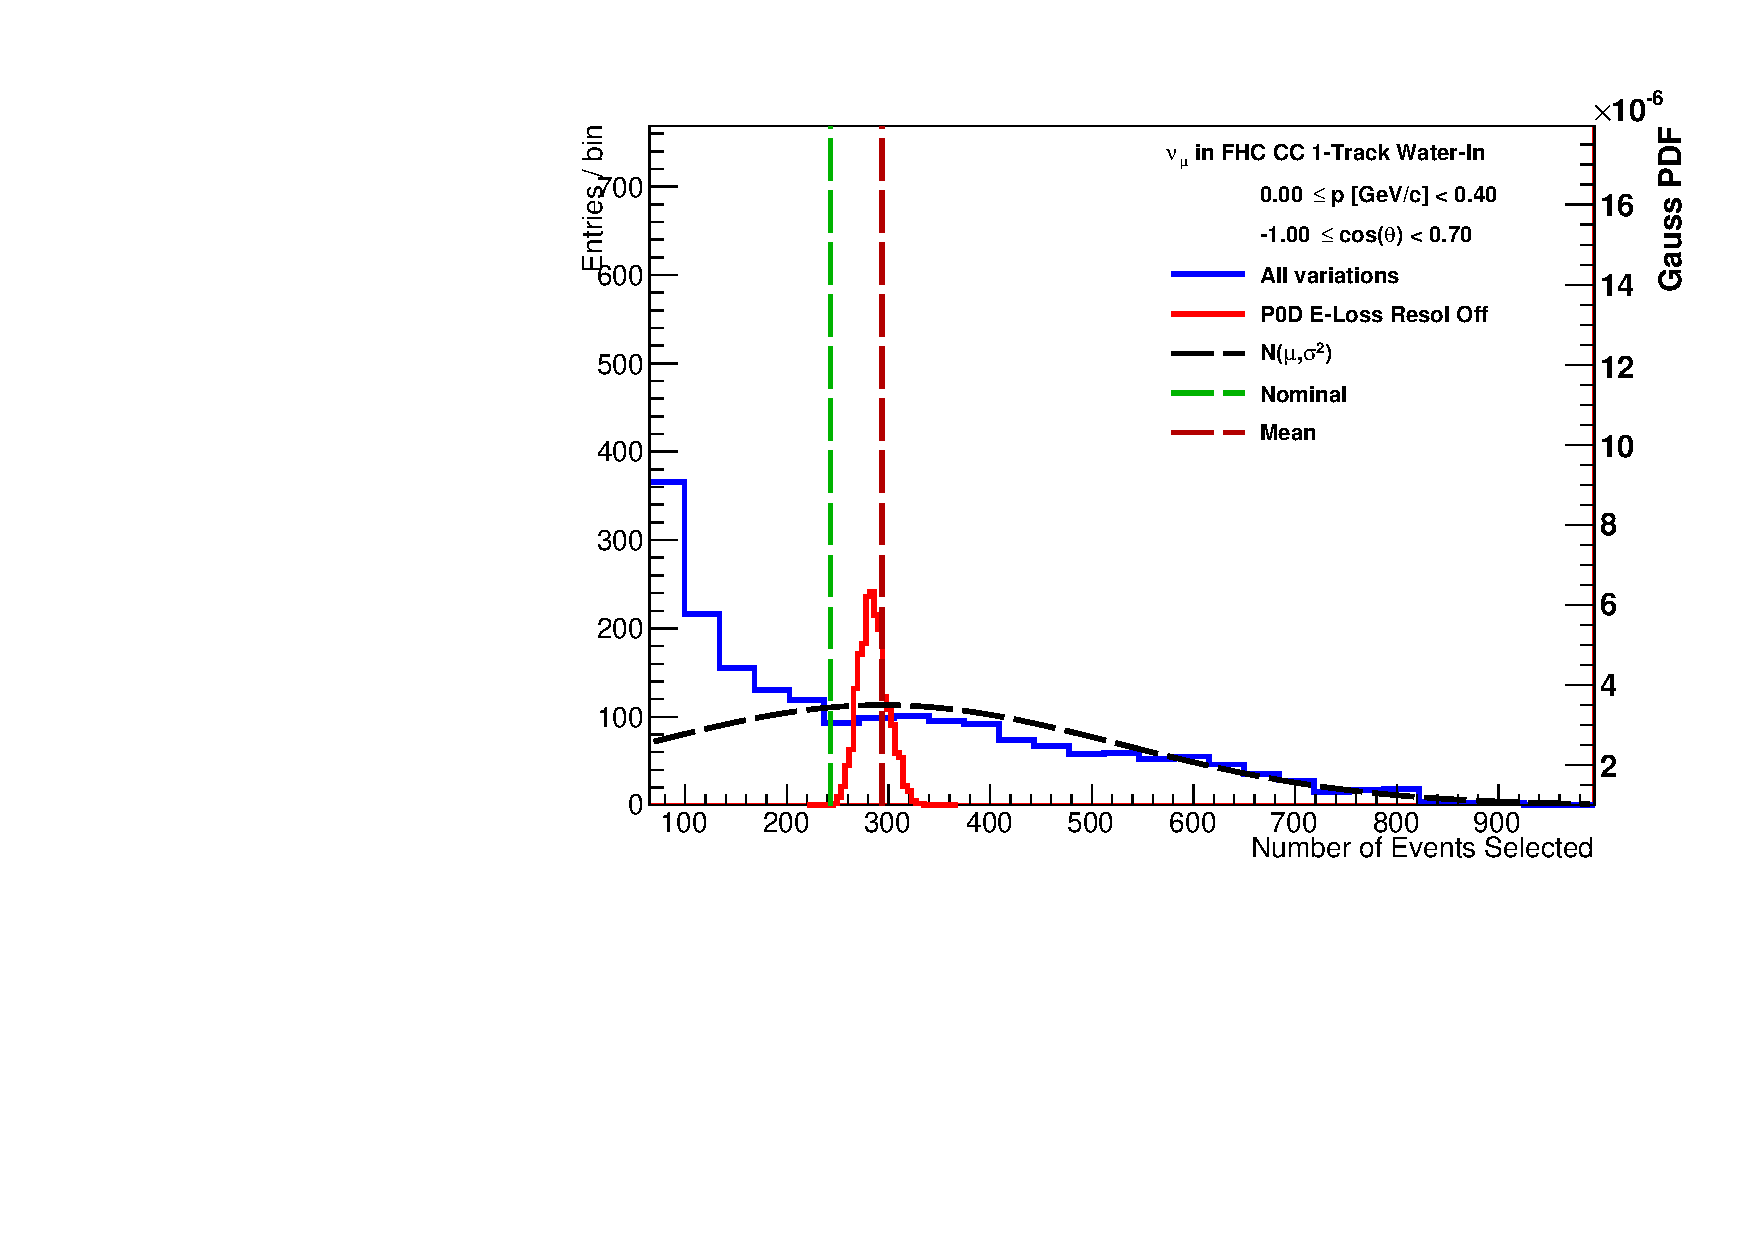
\includepdf[pages=-,nup=3x6,pagecommand=\thispagestyle{plain},width=2in]{Appendices/Figures/ToyExperiments/P0DObsnorms_all_and_P0DELossResolOff}
